\documentclass[a4paper, 11pt]{report}

\usepackage[german]{babel} % translation of standard elements
\usepackage{blindtext}

\usepackage{multicol} % allow arbitrary number of columns

\usepackage{xspace} % context sensitive space after command
\usepackage[dvipsnames, table]{xcolor}

\usepackage{fancyhdr}
\usepackage{lastpage}

\usepackage[left=2cm, right=2cm, top=2cm, bottom=3cm]{geometry}

\usepackage{eso-pic,graphicx}

\usepackage{float} % for H setting to include float in multicol

\usepackage{paralist} % compact list

\usepackage{framed}

\usepackage{csvsimple}
\usepackage{listofitems}
\usepackage{etoolbox}

\usepackage{microtype} % helps with justification

\usepackage[backend=bibtex,style=verbose-trad2]{biblatex}

\usepackage{hyperref}

\usepackage{vhistory} % version history

\usepackage{enumitem} % allows nolistsep, noitemsep to reduce spacing in listings

\hypersetup{
	hidelinks=true,
	colorlinks,
	allcolors=Blue
}

\pagestyle{fancy}
\fancyhf{}
\lhead{\nouppercase{\leftmark}}
\rhead{\nouppercase{\rightmark}}
\rfoot{Seite \thepage \hspace{1pt} von \pageref{LastPage}}
\lfoot{\gdocname}

\fancypagestyle{plain}{ % this is used to redefine 'plain' pages like table of contents
	\fancyhf{}
	\lhead{\nouppercase{\leftmark}}
	\rhead{\nouppercase{\rightmark}}
	\rfoot{Seite \thepage \hspace{1pt} von \pageref{LastPage}}
	\lfoot{\gdocname}
}

\newcommand{\docname}[1]{\renewcommand{\gdocname}{#1}}
\newcommand{\gdocname}{DOCNAME REQUIRED!}

\newcommand{\warnlabel}[1]{\fbox{\color{YellowOrange}\textbf{#1}}\\}

\newcommand{\unimplemented}{\warnlabel{Feature eingeplant aber unimplementiert in aktueller Version}}

\docname{Astrodynamics} % document name for footer
\title{Astrodynamics\\
	\large{Anleitung und Dokumentation}\\
	\small{Version \vhCurrentVersion}}
\author{Marc Singer, Rafael Stauffer}
\date{\vhCurrentDate}
\bibliography{citations}

\begin{document}
	\maketitle
	\begin{versionhistory}
	\vhEntry{0.1}{21.01.2023}{RS}{Erstellung}
\end{versionhistory}
	\tableofcontents
	\chapter{Ziel und Zweck}

Dieses Projekt hat das Ziel die teilweise kontraintuitiven Gesetzmässigkeiten welche im Weltraum gelten greifbar zu machen.
Der Author der primären Inspirationsquelle ''Children of a Dead Earth''\footcite{COADE:1} schreibt dazu passend:
\begin{quote}
	For me, though, I wanted a simulation, one that was actually based on real equations. This is because in my experience, whenever you develop system this complex, it tends to surprise you, and will often overturn your assumptions.
\end{quote}

Da wir als Team bisher keine Erfahrungen im Bereich von Physiksimulationen hatten wurde als Ziel die Realisierung einer N-Körper-Simulation festgelegt welche zukünftig erweitert werden kann.

%\begin{quotation}
%	What is “human”?
%	In the year 2100, humanity faces its greatest challenge: settling the vast reaches of the solar system. %Spacegoing transnationals develop technologies that governments fear to explore, while bizarre posthuman %cultures bloom like exotic flowers. Will “human” cease to have any meaning in a world of genetic engineering %and digital consciousness?
%\end{quotation}
%Klappentext des Transhuman Space Regelbuchs\footcite{SJGTHS:1}.


	\chapter{Benutzeranleitung}

\hypertarget{missionlist}{\section{Missionsliste}}

\begin{figure}[H]
	\centering
	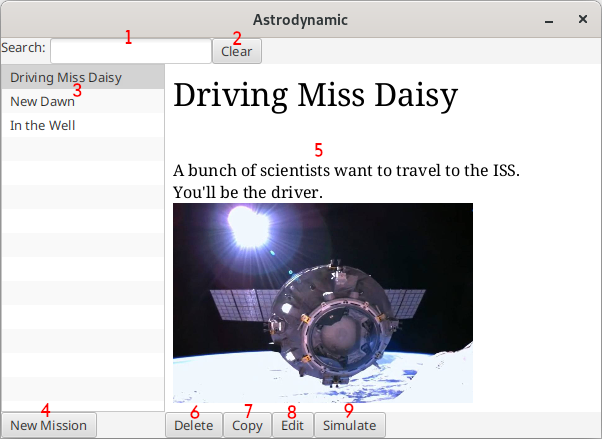
\includegraphics[width=12cm]{res/missionsliste.png}
	\caption{GUI Missionsliste mit Annotation}
\end{figure}

\begin{enumerate}[noitemsep]
	\item Suchfeld
	\item Clear: Suchfeld leeren
	\item Liste verfügbarer Missionen
	\item New Mission: Neue Mission öffnen im Missions-Editor
	\item Beschreibung der ausgewählten Mission
	\item Delete: Ausgewählte Mission löschen
	\item Copy: Ausgewählte Mission kopieren
	\item Edit: Ausgewählte Mission öffnen im Missions-Editor
	\item Simulate: Ausgewählte Mission öffnen im Simulator
\end{enumerate}

\subsection{Grundlagen}
Die Missionsliste ist der Einstiegsbildschirm beim Start des Programs.
Hat der Benutzer keine Mission gespeichert welche geladen werden kann so werden drei Testmissionen geladen.
Am linken Rand befindet sich die Liste der verfügbaren Missionen.Anwählen einer Mission in der Liste per Klick mit der Linken Maustaste lädt die Missionsbeschreibung in den rechten Anzeigebereich und ermöglicht mit diese Mission per Buttons unten rechts am Bildschirmrand weiter zu Interagieren.

\subsection{Missionen nach Beschreibung suchen}
Das Suchfeld führt eine sofortige Textsuche auf Missions-Name und -Beschreibung durch und zeigt auf Basis dieser nur passende Missionen in der Liste der verfügbaren Missionen. Durch drücken des Clear-Buttons können längere Sucheingaben sofort gelöscht und die Sortierung zurückgesetzt werden.

\begin{figure}[h]
	\centering
	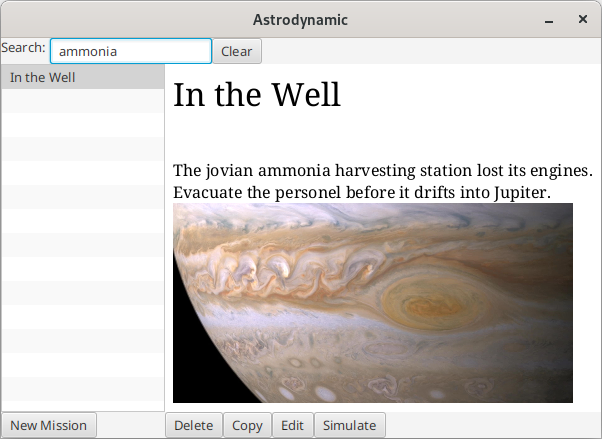
\includegraphics[width=8cm]{res/search.png}
	\caption{Missionsfilter bei Suche nach 'ammonia'}
\end{figure}

\subsection{Anlegen einer neuen Mission}
Klicken sie auf den ''Neue Mission öffnen im Missions-Editor''-Button unten links.
Es öffnet sich nun der Missions-Editor.
Für Details zum editieren einer Mission konsultieren sie das \hyperlink{missioneditor}{Kapitel Missions-Editor}.

\subsection{Löschen einer Mission}
Wählen sie die Mission aus der Liste der verfügbaren Missionen per Mausklick aus.
Klicken sie auf Delete.
Ein Popup öffnet sich mit der Löschanfrage.

\begin{figure}[H]
	\centering
	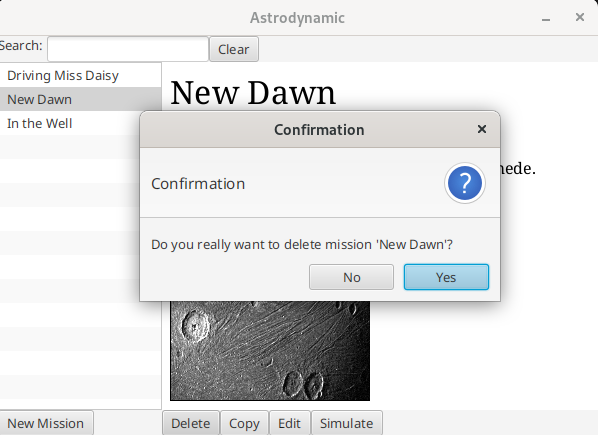
\includegraphics[width=8cm]{res/loeschen.png}
	\caption{Sicherheitsabfrage bei Missionslöschung}
\end{figure}

Bestätigen sie das Popup mit Klick auf Yes.
Die Mission wird aus der Liste der verfügbaren Missionen entfernt.

\subsection{Kopieren einer Mission}
\unimplemented
Wählen sie die Mission aus der Liste der verfügbaren Missionen per Mausklick aus.
Klicken sie auf Copy.
Es öffnet sich nun der Missions-Editor mit der kopierten Mission.
Für Details zum editieren einer Mission konsultieren sie das \hyperlink{missioneditor}{Kapitel Missions-Editor}.

\subsection{Editieren einer Mission}
Wählen sie die Mission aus der Liste der verfügbaren Missionen per Mausklick aus.
Klicken sie auf Edit.
Es öffnet sich nun der Missions-Editor mit der ausgewählten Mission.
Für Details zum editieren einer Mission konsultieren sie das \hyperlink{missioneditor}{Kapitel Missions-Editor}.

\subsection{Simulieren einer Mission}
Wählen sie die Mission aus der Liste der verfügbaren Missionen per Mausklick aus.
Klicken sie auf Simulate.
Es öffnet sich nun der Simulator mit der ausgewählten Mission.
Für Details zum simulieren einer Mission konsultieren sie das \hyperlink{simulator}{Kapitel Simulator}.
	\hypertarget{missioneditor}{\section{Missions-Editor}}

\begin{figure}[H]
	\centering
	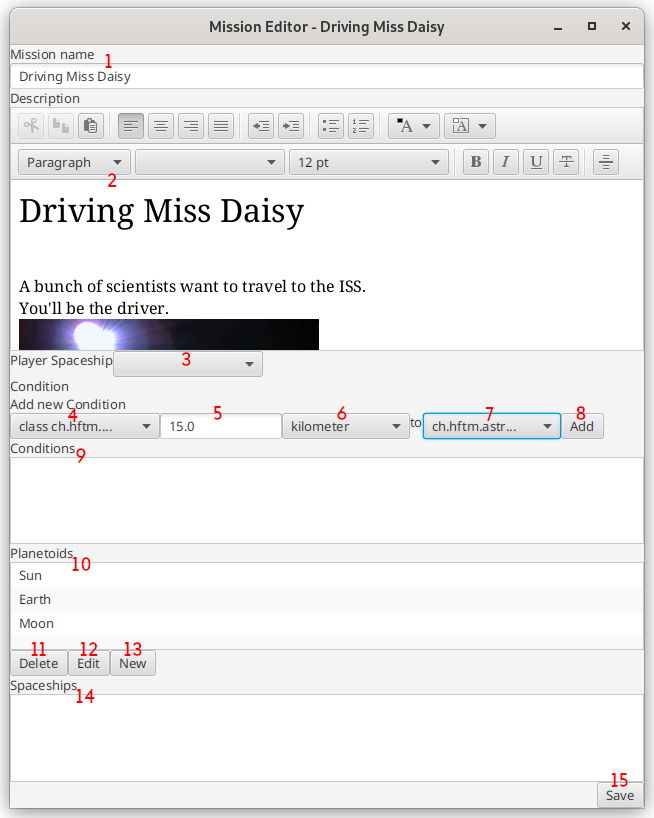
\includegraphics[width=12cm]{res/missioneditor.png}
	\caption{GUI Mission-Editor mit Annotation. Testmission 'Driving Miss Daisy' geöffnet.}
\end{figure}

\begin{enumerate}[noitemsep]
	\item Missionsname
	\item Missionsbeschreibung HTML-Editor
	\item Auswahl Spielerraumschiff
	\item Missionsbedingung: Bedingungstyp-Dropdown
	\item Missionsbedingung: Zahlenfeld
	\item Missionsbedingung: Masseinheit-Dropdown
	\item Missionsbedingung: Referenzobjekt-Dropdown
	\item Missionsbedingung hinzufügen
	\item Missionsbedingungen-Liste
	\item Planetoiden-Liste
	\item Planetoid entfernen
	\item Planetoid editieren
	\item Planetoid hinzufügen
	\item Raumschiff-Liste
	\item Missionsänderungen speichern
\end{enumerate}

\subsection{Grundlagen}
Der Missions-Editor erlaubt das Ändern des Missions-Namen und Beschreibung. Durch das Hinzufügen von Missionsbedingungen, auch Conditions genannt, können Abbruchsbedinungen für die Simulation festgelegt und weitere dynamische Veränderungen an der Mission vorgenommen werden. Verwendete Planetoiden und Raumschiffe werden in den ensprechenden Listen aufgelistet.

\hypertarget{addcondition}{\subsection{Hinzufügen einer Missionsbedingung}}
Wählen sie im Bedingungstyp-Dropdown den passenden Bedingungstypen.
Siehe \hyperlink{conditiontable}{Abschnitt Missionsbedingen} für eine komplette Liste der möglichen Bedingungstypen, ihren Parametern, und Funktionsweise.
Zahlenfeld, Grössenangabe und Referenzobjekt werden dynamisch ein- oder ausgeblendet.

% nifty way to make two figures side by side
\begin{figure}[H]
	\centering
	\begin{minipage}[b]{0.45\textwidth}
		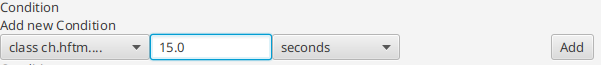
\includegraphics[width=\textwidth]{res/conditionmaxtime.png}
		\caption{MaximumTime}
	\end{minipage}
	\hfill
	\begin{minipage}[b]{0.45\textwidth}
		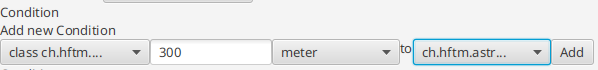
\includegraphics[width=\textwidth]{res/conditionapproach.png}
		\caption{Approach}
	\end{minipage}
\end{figure}

Sollte das Zahlenfeld oder das Referenzobjekt eingeblendet werden so ist eine Eingabe respektive Auswahl zwingend.
Die Masseinheit kann jederzeit geändert werden, ein valider Wert im Zahlenfeld wird in die neue Einheit umgewandelt.

\begin{figure}[H]
	\centering
	\begin{minipage}[b]{0.45\textwidth}
		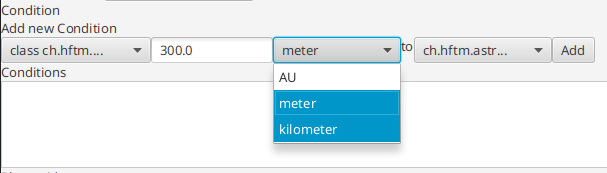
\includegraphics[width=\textwidth]{res/conditionunits.png}
		\caption{Masseinheit Meter}
	\end{minipage}
	\hfill
	\begin{minipage}[b]{0.45\textwidth}
		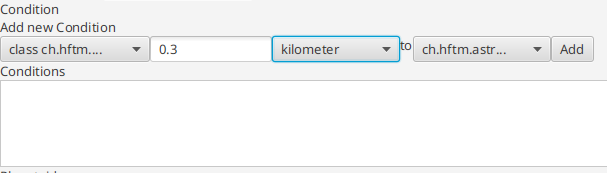
\includegraphics[width=\textwidth]{res/conditionunits2.png}
		\caption{Masseinheit Kilometer}
	\end{minipage}
\end{figure}

Klicken sie auf den Add-Button um die Missionsbedingung hinzuzufügen.
Die Missionsbedingung wird nun in der Missionsbedingungen-Liste aufgeführt.

\begin{figure}[H]
	\centering
	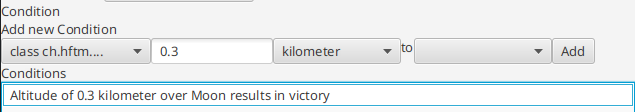
\includegraphics[width=0.45\textwidth]{res/conditionadded.png}
	\caption{Neue Approach-Missionsbedingung hinzugefügt}
\end{figure}

\hypertarget{conditiontable}{\subsection{Missionsbedingungen}}

\begin{table}[H]
	\centering
	\begin{tabular}{ || m{3cm} | m{5cm} | m{8cm} || }
		\hline
		\textbf{Bedingung} & \textbf{Parameter} & \textbf{Funktionsweise} \\
		\hline
		\hline
		MaximumTime & Zeitwert & Mission gilt als Fehlschlag wenn Missionsdauer den Zeitwert überschreitet \\
		\hline
		HoldoutTime & Zeitwert & Mission gilt als Gewonnen wenn Missionsdauer den Zeitwert überschreitet \\
		\hline
		Approach & Distanz und Referenzobjekt & Mission gilt als Gewonnen wenn Spielerraumschiff die maximale Distanz zum Referenzobjekt erreicht oder unterschreitet \\
		\hline
		Avoid & Distanz und Referenzobjekt & Mission gilt als Fehlschlag wenn Spielerraumschiff die maximale Distanz zum Referenzobjekt erreicht oder unterschreitet \\
		\hline
		Depart & Distanz und Referenzobjekt & Mission gilt als Gewonnen wenn Spielerraumschiff die minimale Distanz zum Referenzobjekt erreicht oder überschreitet \\
		\hline
		SetupHeavyLander & Distanz und Referenzobjekt & Platziert das Raumschiff 'Heavy Lander' in ein Orbit um Referenzobjekt mit Höhe von Distanz\\
		\hline
		SetupISS & Distanz und Referenzobjekt & Platziert das Raumschiff 'ISS' in ein Orbit um Referenzobjekt mit Höhe von Distanz\\
		\hline
	\end{tabular}
	\caption{Verfügbare Missionsbedingungem}
\end{table}

\subsection{Löschen eines Planetoiden}
Wählen sie den zu löschenden Planetoiden mit einem Klick aus der Planetoiden-Liste aus.
Klicken sie den Delete-Button.
Es öffnet sich eine Sicherheitsabfrage.

\begin{figure}[H]
	\centering
	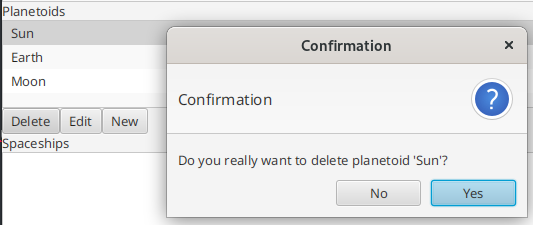
\includegraphics[width=0.45\textwidth]{res/loeschenplanetoid.png}
	\caption{Sicherheitsabfrage bei Planetoidenlöschung}
\end{figure}

Bestätigen sie das Popup mit Yes.
Der Planetoid ist nun aus der Mission entfernt und die Planetoiden-Liste aktualisiert worden.

\subsection{Editieren eines Planetoiden}
Wählen sie den zu editierenden Planetoiden mit einem Klick aus der Planetoiden-Liste aus.
Klicken sie auf den Edit-Button.
Es öffnet sich nun der Planetoid-Editior mit dem ausgewählten Planetoiden.
Für Details zum Planetoid-Editior konsultieren sie das \hyperlink{planetoideditor}{Kapitel Planetoid-Editior}.

\subsection{Hinzufügen eines Planetoiden}
Klicken sie auf den New-Button unterhalb der Planetoiden-Liste.
Es öffnet sich nun der Planetoid-Editior.
Für Details zum Planetoid-Editior konsultieren sie das \hyperlink{planetoideditor}{Kapitel Planetoid-Editior}.

\subsection{Hinzufügen eines Raumschiffs}
Zum hinzufügen eines Raumschiffs benutzen sie die Condition 'SetupHeavyLander'.
Siehe \hyperlink{addcondition}{Abschnitt Hinzufügen einer Missionsbedingung}.
	\hypertarget{planetoideditor}{\section{Planetoid-Editor}}
	\hypertarget{simulator}{\section{Simulator}}

\begin{figure}[H]
	\centering
	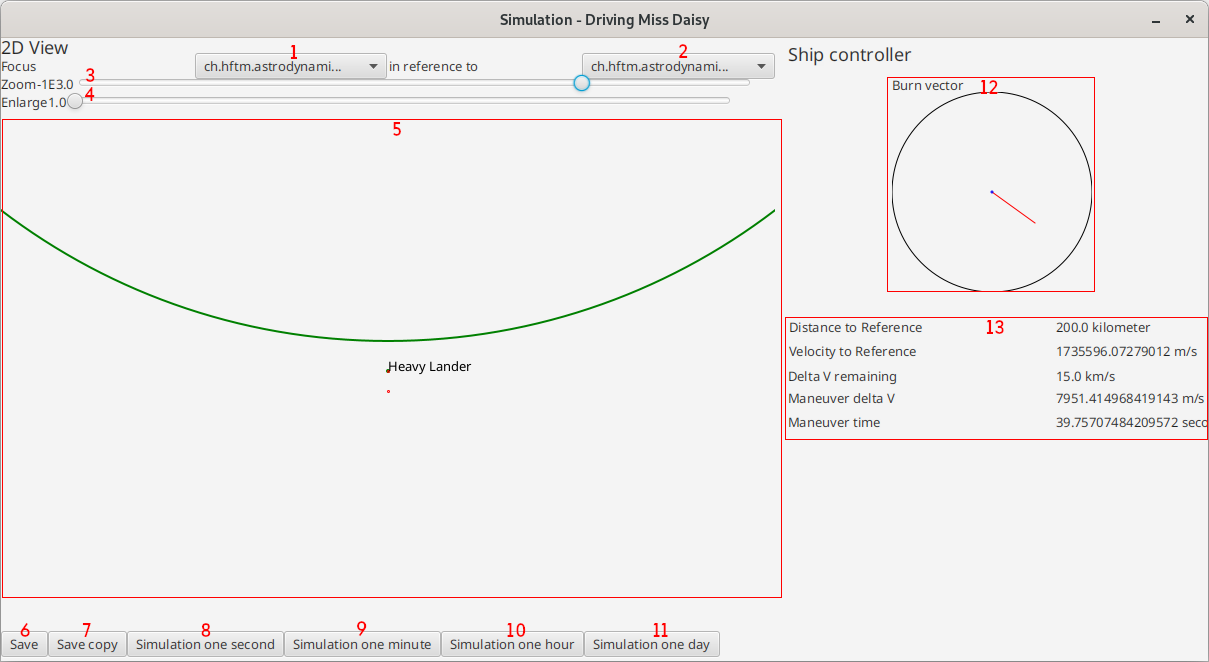
\includegraphics[width=\textwidth]{res/simulation.png}
	\caption[GUI Simulation mit Annotation]{GUI Simulation mit Annotation. Heavy Lander im Fokus, ISS als Referenz}
\end{figure}

\begin{enumerate}[noitemsep]
	\item Fokus-Objekt
	\item Referenz-Objekt
	\item Zoom
	\item Objektvergrösserung
	\item Orbital-View
	\item Save: Speichern der Simulation
	\item Save copy: Kopieren der Simulation
	\item Simulation eine Sekunde berechnen
	\item Simulation eine Minute berechnen
	\item Simulation eine Stunde berechnen
	\item Simulation einen Tag berechnen
	\item Burn vector: Maneuver-Darstellung
	\item Informationspanel
\end{enumerate}

\subsection{Grundlagen}
Der Simulator erlaubt eine simple graphische Darstellung der Simulation. Die linke Seite des Fensters wird dabei von der Orbital-View, auch 2D-View genannt, eingenommen welche ein ortographisches Bild der Objekte darstellt. Mit Zoom und Objektvergrösserung können kleinere und grössere Objekte aufgefunden und zentriert werden. Die rechte Seite des Fensters wird beim Fokus eines Raumschiffs mit der Maneuver-Darstellung welche das geplante Maneuver graphisch darstellt sowie dem Informationspanel gefüllt.

\subparagraph{Maneuver-Vektor}
Der schwarze Kreis stellt die maximal verfügbare Geschwindigkeitsänderung welche das aktuell fokussierte Raumschiff durchführen kann dar. Bei einem aktiven Maneuver wird eine rote Linie in die Richtung in welche die Geschwindigkeitsänderung durchgeführt wird gezogen. Die Linienlänge stellt den benötigten Wert an Geschwindigkeitsänderung gegenüber dem verfügbaren Vorrat (schwarzer Kreis) dar und ändert sich deshalb bei der Durchführung des Maneuvers. Ein Befehl über dem verfügbaren Vorrat ist möglich, es wird jedoch nur bis zum verfügbaren Vorrat durchgeführt.

\subsection{Navigieren im Orbital-View}


\subsection{Ausführen eines Maneuvers}
Fokusieren sie ein Raumschiff.
Klicken sie in den schwarzen Kreis der Maneuver-Darstellung.
Eine rote Linie vom Zentrum zu ihrer angeklickten Position erscheint.
Auf dem Informationspanel wird die geplante Geschwindigkeitsänderung (Bezeichnung \emph{Maneuver delta V}) und die Zeitdauer zum Durchführen des Maneuvers (Bezeichnung \emph{Maneuver time}) angegeben.\\
Klicken sie nun auf einen beliebigen Simulationsbutton bis die Zeitdauer in der Simulation vergangen ist.
Während der Simulation verändert sich die Länge des Maneuver-Vektors u
	\chapter{Technische Dokumentation}

\section{Applikationsdokumentation}

\subsection{Diagramme}

\begin{figure}[H]
	\centering
	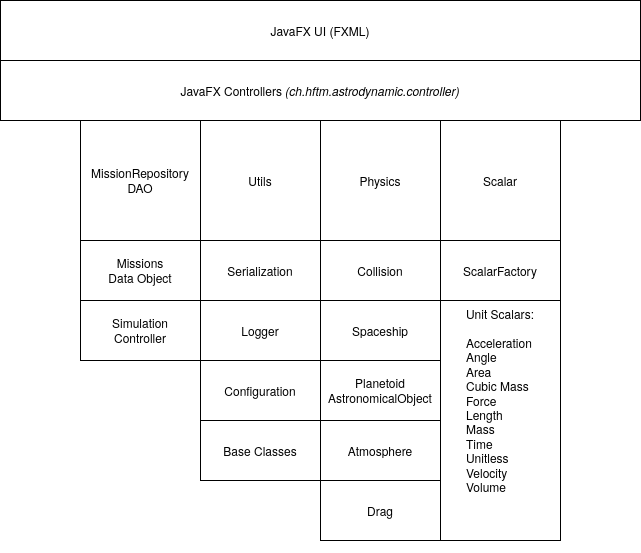
\includegraphics[width=12cm]{res/overview.png}
	\caption{Übersicht Aufbau Astrodynamic}
\end{figure}

\begin{figure}[H]
	\centering
	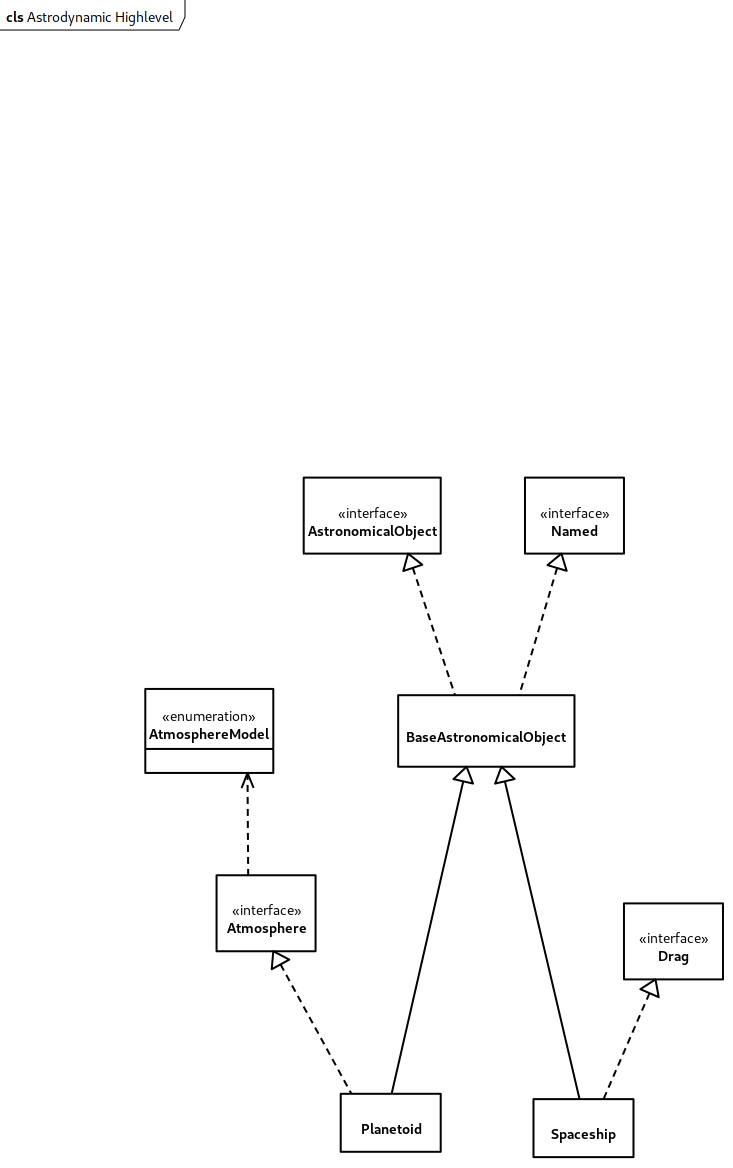
\includegraphics[width=12cm]{res/AstrodynamicHighlevel.png}
	\caption{Übersicht Physik-Klassen und -Interfaces}
\end{figure}

Das BaseAstronomicalObject bietet die Basis für die Physikberechnung. Spezifische Interfaces wie die Atmosphärendaten für die Planeten oder Drag-Berechnungen für die Raumschiffe werden in den jeweiligen Kindklassen implementiert.

\begin{figure}[H]
	\centering
	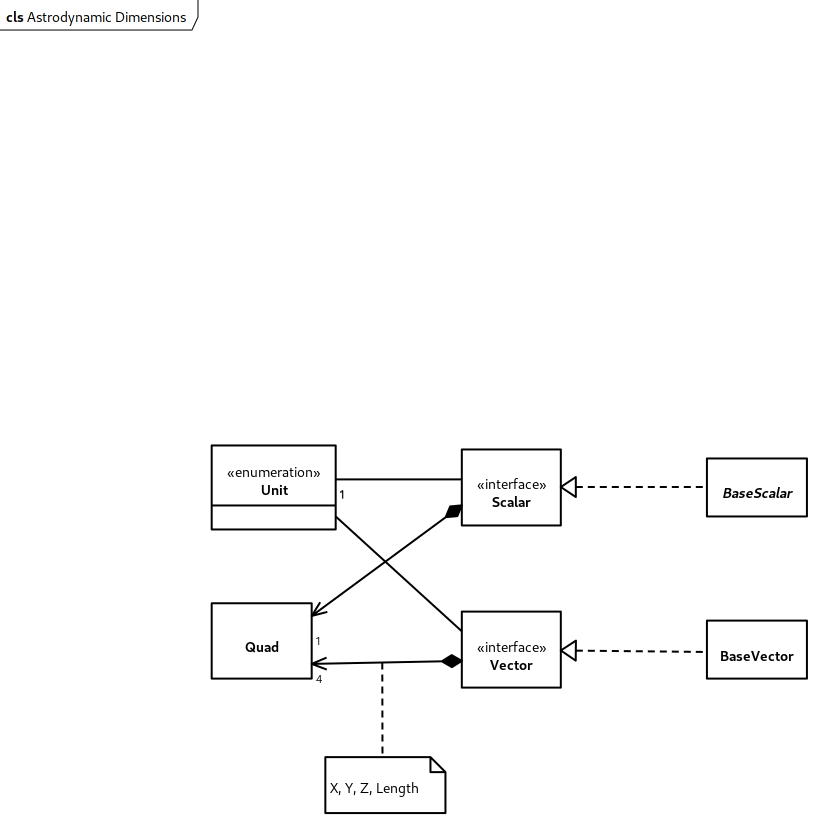
\includegraphics[width=12cm]{res/AstrodynamicDimensions.png}
	\caption{Übersicht Mathematische-Klassen und -Interfaces}
\end{figure}

Scalare und Vektoren verwenden die Quad-Klasse um exakte Werte zu speichern. Um die Dimensionsanalyse in den spezifischen Skalarimplementationen (nicht im Diagram aufgeführt) durchzuführen wird der Enum Unit verwendet.

\begin{figure}[H]
	\centering
	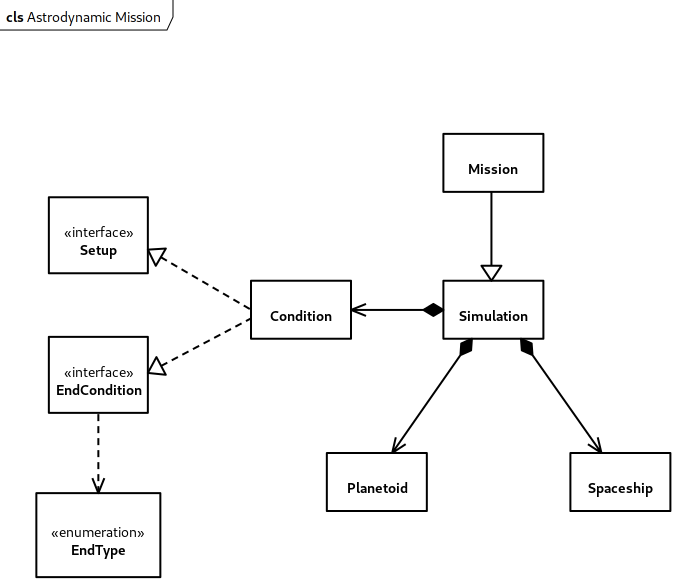
\includegraphics[width=12cm]{res/AstrodynamicMission.png}
	\caption{Übersicht Missions-Klassen und -Interfaces}
\end{figure}

Eine Simulation besteht aus den dazugehörigen Planetoiden und Raumschiffen. Diese sind getrennt verwaltet für einfacheren Zugriff auf spezifische Funktionen, jedoch bietet die Simulation ebenfalls Methoden diese Objekte in einer Liste abzurufen, je nach Ziel und benötigtem Interface.\\
Conditions in der Simulation manipulieren ihren Startzustand und können Abbruchbedingungen definieren und überprüfen.\\
Die Mission stellt einen Wrapper dar welcher weitere Funktionalitäten zur Verfügung stellt welche in einem reinen Simulationskontext nicht benötigt werden.

\subsection{Maven build}

Um mittels Maven ein Build zu erzeugen kann der Befehl \textit{mvn clean package} verwendet werden.

Dieser Befehl testet das gesamte Softwareprojekt und erzeugt anschliessend im Ordner \textit{target} ein neues Java Executable (JAR File).

\subparagraph{Docker}

Wir haben ebenfalls einen Docker Container vorbereitet, mit welchem das Build automatisiert werden kann.

Dieser nutzt das Zulu OpenJDK, um unser Projekt vollständig zu bauen und zu testen:

\begin{lstlisting}

	# Docker build
	$ docker build -t astrodynamic/build .
	$ docker run --name astrodynamic -v ./:/astrodynamic astrodynamic/build
	# Das Java Executable erscheint im selben Ordner
	
\end{lstlisting}

Mit Docker können wir das Projekt überall mit wenig Aufwand und ohne grossen Installationsaufwand neu bauen.

\section{Themenumsetzung}

\subsection{Unit Tests}

Unsere Unit Tests befinden sich im Ordner \textit{src/test/java/ch/hftm/astrodynamic} und sind nach Anwendungskomponenten gegliedert:

\begin{itemize}
	\item DAO (Data Access Object); Testet den Zugriff und die Fuktionalität des zentrale MissionRepositorys (in welchem alle Missionen und deren Kindobjekte gespeichert sind)
	\item Model; Testet die pedefinierten Modelle (z.B Mond, Erde, Sonne) welche mit der Software mitgeliefert werden
	\item Planetoid; Testet die Funktionalität der Planetoiden (also planetenähnlichen Objekten)
	\item Quad; Testet die Implementation und Abstraktion unseres Quad Datentyps, welcher für alle Berechnungen innerhalb des Projekts verwendet wird
	\item Scalar; Testet die Richtigkeit von Scalar basierten Verrechnungen
	\item SimulationTest; Testet die Simulation der einzelnen Objekte im Sonnensystem
	\item Unit; Testet die verschiedenen Scalar Physik-Einheiten und deren Verrechnungen
	\item Vector; Testet die Vektoren und deren Verrechnungen
\end{itemize}

Wir haben uns primär dafür entschieden, die Business-Logik (primär die Simulation) zu testen, da die Erfolg unseres Projekts primär von der Korrektheit der Simulation abhängig ist.

\subparagraph{Unit Tests ausführen}

Zunächst müssen wir uns ins \textit{astrodynamics} Verzeichnis bewegen in welchem ebenfalls die Datei \textit{pom.xml} gespeichert ist.
Anschliessend können wir die Unit-Tests mit einem einfachen \textit{mvn clean test} ausführen.

\subsection{Enumeration}

Unser wichtigster Einsatz von Enum (Enumeration) findet in der Klasse \textit{Unit} statt. Diese Klasse wird dazu genutzt, SI Einheiten, welche in unserem Projekt verwendet werden, darzustellen:

\begin{lstlisting}
	
	// Contains all physical units as enum
	public enum Unit {
		TIME, // Seconds (s)
		LENGTH, // Meters (m)
		MASS, // Kilogram (kg)
		CURRENT, // Ampere (A)
		TEMPERATURE, // Kelvin (K)
		MOLECULES, // Mol (mol)
		LUNINOSITY, // Candela (cd)
		// Extensions (Implicit)
		VOLUME,  // m ^ 3
		AREA, // m ^ 2
		FORCE, // N
		ACCELERATION, // m/s ^ 2
		VELOCITY, // m/s
		ANGLE, // radian
		ANGULAR_VELOCITY, // radian/second
		ANGULAR_ACCELERATION, // radian/second^2
		// kg ^ 2 imaginary unit for gravitational calculations
		CUBIC_MASS, 
		// kg ^ 2 / m ^ 2 imaginary unit for gravitational calculations
		M2_DIV_L2,
		// N * m ^ 2 * kg ^ 2 gravitational constant
		//  (s ^ -2 * m ^ 3 * kg ^ - 1) 
		F_L2_Mn2,
		// Unitless for scalars without unit
		UNITLESS
	}

\end{lstlisting}

Wir nutzen dieses Enum in allen Skalaren und in diversen Vektoren, um die Einheiten der Werte darzustellen. z.B nutzt die Klasse \textit{LengthScalar}, welche eine Länge speichert, den Wert \textit{LENGTH}.

In den Kommentaren der Klasse werden die genauen Einheiten explizit definiert. Dies hilft bei den Umrechnungen der Werte z.B zwischen verschiedenen Zeiteinheiten (z.B zwischen Stunden, Tagen oder Wochen).

\section{Vererbung}

Wir nutzen Vererbung in allen unseren Klassen. Spezifisch hervorheben möchten wir in diesem Fall die \textit{Scalar} Klassen im Package \textit{ch.hftm.astrodynamic.scalar}, welche allesamt von der Klasse \textit{BaseScalar} im Package \textit{ch.hftm.astrodynamic.utils} erben.

Die einzelnen \textit{Scalar} Klassen stellen jeweils einen spezialisierten Scalar im Projekt dar. z.B werden Längen mittels dem \textit{LengthScalar} dargestellt.
Die Einheiten der jeweiligen Klassen werden in der Kind-Klasse innerhalb des Konstruktors statisch gesetzt und dem Eltern-Konstruktor des \textit{BaseScalar} übergeben und gespeichert.

\section{Casting}

Da wir für die Serialisierung einen eigenen Serializer / Deserializer innerhalb der Klasse \textit{MissionRepository} in \textit{ch.hftm.astrodynamic.utils} implementieren mussten (die Klasse \textit{ObservableList} ist nicht Serialisierbar), verwenden wir Casting in diesem Fall für die Konvertierung zwischen \textit{Object} und \textit{Mission}.

Casting wird ausserdem in einzelnen Fällen innerhalb der Controller verwendet, um z.B einen Double zu einem Integer zu Runden.

\section{Interfaces}

Interfaces werden in unserem Projekt häufig verwendet. Vorwiegend haben wir mittels Interfaces generalisierte Klassen (und deren Vererbungen) implemtiert.

Als Beispiel dient hier das Interface \textit{Scalar} aus dem Package \textit{ch.hftm.astrodynamics.utils}, welches z.B für generalisierte Operationen innerhalb aller Klassen verwendet wird. Mit diesem Interface können wir sicherstellen, dass alle \textit{Scalar} Klassen verglichen oder berechnet werden können.

Ebenfalls ist in diesem Interface eine Implementation für die Funktion \textit{toFittedString()} bereits vorgegeben (und muss aus diesem Grund nicht erneut implementiert werden).

\section{Abstrakte Klassen}

Wir nutzen Abstrakte Klassen unter anderem für unseren \textit{BaseController} im Paket \textit{ch.hftm.astrodynamic.controller} welcher grundlegende Funktionalität für unsere Controller bereitstellt.

Dieser Controller dient als Elternklasse für unsere \textit{Controller} Klassen, wird aber selbst niemals instanziert (daher ist er als Abstract definiert).

Wir verwenden abstrakte Klassen ebenfalls für die \textit{Condition} Klasse für die Mission aus demselben Grund.

\section{Collection}

Der wichtigste Einsatz von Collections in unserem Projekt ist die \textit{ObservableList} innerhalb unseres MissionRepositories.
Dieser Typ der Collection stammt aus dem JavaFX Paket und bietet der Frontend-Anwendung die Möglichkeit, den Inhalt der Liste konstant zu überwachen und Änderungen im UI umgehend darzustellen.


\subparagraph{Sortierung}

Wir sortieren die \textit{ObservableList} innerhalb der Funktion \textit{sort()} innerhalb unserer Klasse \textit{MissionRepository} alphabetisch nach Namen der Mission:


\begin{lstlisting}
	// Sorts the MissionRepository alphabetically
	public static void sort() {
		// Create a comparator for name based sorting 
		Comparator<Mission> byName = (Mission a, Mission b) ->
		a.getName().compareTo(b.getName());
		// Sort the Mission Repository based on names
		getInstance().missions.sort(byName);
	}
\end{lstlisting}

Der Name ist ebenfalls der Primärschlüssel, welcher für die Missionen innerhalb der Funktion \textit{getMissionByName} verwendet wird.

\section{Serialisierung}

Serialisierung wird in unserem Projekt zur Speicherung der Klasse \textit{MissionRepository}, welche den kompletten Status unserer Anwendung enthält verwendet.

Die Klasse \textit{Serializer} ist für die Serialisierung des \textit{MissionRepository} zuständig.
Aktuell wird die Serialisierbarkeit unserer Klassen mittels dem Interface \textit{Serializable} gewährleistet.
Dies ist insbesondere für die Komplexen Datentypen, welche für \textit{Quad} und \textit{ObservableList} verwendet werden, wichtig.
Da \textit{ObservableList} das Interface \textit{Serializable} nicht implementiert, musste im \textit{MissionRepository} mittels der Funktionen \textit{WriteObject()} und \textit{ReadObject()} die Missionen in ein Array konvertiert werden. Dieses Array wird beim Deserialisieren wiederum in Missionen gecasted, welche dem \textit{MissionRepository} hinzugefügt werden.

Ebenfalls wurde eine mögliche Serialisierung ins JSON-Format vorbereitet. Dazu verwenden wir die Bibliothek \textit{Jackson}, welche ebenfalls in diversen Java Web Bibliotheken verwendet wird und als performant gilt.

\section{Speichern und Laden der Missionen}

\subparagraph{Laden}
Beim Start der Anwendung werden die gespeicherten Missionen aus einer Datei geladen.
Der Pfad dieser Datei kann mittels der Konfiguration \textit{STATE FILE} angepasst werden.
Der Standardname der Datei lautet: \textit{state.bin}.
Diese Datei kann ebenfalls gelöscht werden, um den Ursprungszustand wiederherzustellen.

\subparagraph{Speichern}
Wenn Missionen geändert werden, werden diese automatisch in die (aktuell konfigurierte) Projektdatei geschrieben.


\section{Exceptions}

Mit dem \textit{UnitConversionError} im \textit{ch.hftm.astrodynamic.utils} Package haben wir unsere eigene Exception implemementiert.
Diese Exception dient dazu, inkompatible Einheiten in den \textit{Scalar} Klassen abzufangen und zu handeln.
Ebenfalls nutzen wir mit dem \textit{SimulationRuntimeError} eine weitere eigene Exception, welche für Fehler während der Simulation genutzt wird.

\section{Logging}

Wir nutzen unseren eigenen Logger, welchen wir innerhalb der Klasse \textit{Log} in \textit{ch.hftm.astrodynamic.utils} implementiert haben.
Diese Klasse konfiguriert den Logger basierend auf Konfigurationswerten aus der Klasse \textit{ConfigRepository}.
Um den Logger zu nutzen kann die Methode \textit{build()} verwendet werden, welche den konfigurierten Logger des Typs \textit{java.util.logging.Logger} zurückgibt.

\subparagraph{Levels}

Mittels dem Konfigurationswert \textit{LOG LEVEL} kann der Level des Log Outputs definiert werden.
Die Standardkonfiguration für das Level ist auf \textit{INFO} gesetzt. Mit diesem Level werden alle Meldungen mit höherer Priorität als Info ausgegeben. 

\subparagraph{File}

Mittels dem Konfigurationswert \textit{LOG FILE} kann ein Log File definiert werden, in welchen die Logzeilen gespeichert werden.
In der Standardkonfiguration wird das Logfile \textit{astrodynamic.log} verwendet.

\section{Pakete}

Wir strukturieren unser Projekt innerhalb verschiedenen Java Paketen:

\begin{itemize}
	\item controller; Enthält alle Controller für das Frontend
	\item gui; Enthält Komponenten, welche im Frontend verwendet werden
	\item model; Enthält Modelle für die Simulation
	\begin{itemize}
		\item conditions; Enthält Bedingungen für Missionen
		\item planetoids; Enthält vordefinerte Planeten für Missionen
		\item spaceships; Enthält vordefinierte Weltraumfahrzeuge für Missionen
	\end{itemize}
	\item physicts; Enthält Klassen für physikalische Objekte
	\item scalar; Enthält Kinder-Klassen für Scalare (Werte mit zugewiesenen Einheiten)
	\item utils; Enthält Hilfsklassen und Basisklassen
	\item ressources; Enthält Ressourcen (z.B Bilder), welche in unserem Projekt verwendet werden 
\end{itemize}

Diese Pakete können einzeln oder ganz innerhalb des Projekts oder anderen Projekten importiert werden.

\section{Singletons}

Wir nutzen in unserem Projekt Singleton Klassen, um sicherzustellen, dass nur ein einzelnes statisches Element veränderbar ist.

Ein Beispiel einer solchen Klasse ist das \textit{MissionRepository} aus dem Paket \textit{ch.hftm.astrodynamic.utils}.
Die integrierte \textit{ObservabeList missions} muss für das gesamte Projekt während der Laufzeit einmalig sein. Damit wir keine Instanzen übergeben müssen, instanzieren wir diese Liste statisch.

Während die Liste selbst statisch bleibt, kann das MissionRepository jederzeit instanziert werden.

	\printbibliography
	\addcontentsline{toc}{chapter}{Literatur} % add Bibliography as chapter in table of contents
	\listoffigures
	\addcontentsline{toc}{chapter}{Abbildungsverzeichnis}
	\listoftables
	\addcontentsline{toc}{chapter}{Tabellenverzeichnis}
\end{document}